\documentclass[a4paper,12pt]{article}
\usepackage[utf8]{inputenc}
\usepackage[ngerman]{babel}
\usepackage{amsmath}
\usepackage{mathtools}
\usepackage{float}
\usepackage{listings}
\usepackage{color}
\usepackage{graphicx}
\graphicspath{ {./pics/} }

\definecolor{pblue}{rgb}{0.13,0.13,1}
\definecolor{pgreen}{rgb}{0,0.5,0}
\definecolor{pred}{rgb}{0.9,0,0}
\definecolor{pgrey}{rgb}{0.46,0.45,0.48}

\lstdefinestyle{dsl}{
	 morekeywords={with, subproxy, structproxy, for, simpleproxy, contentproxy, containerproxy, nominalproxy, provided, required, interface, extends, inject, in, posModi},
  showspaces=false,
  showtabs=false,
  breaklines=true,
   literate=
               {-->}{$\rightarrow{}$}{1}
               ,
  showstringspaces=false,
  breakatwhitespace=true,
  commentstyle=\color{pgreen},
  keywordstyle=\color{pblue},
  stringstyle=\color{pred},
  basicstyle=\fontsize{9}{10}\selectfont\ttfamily,
  moredelim=[il][\textcolor{pgrey}]{$ $},
  moredelim=[is][\textcolor{pgrey}]{\%\%}{\%\%}
}




\newcommand{\matchTyp}[3]
{
#1  
\Rightarrow_{#2}
 #3
}

\begin{document}



\section{Beispiel-Bibliothek}



\begin{lstlisting}[style = dsl]
provided Fire extends Object{}
\end{lstlisting}

\begin{lstlisting}[style = dsl]
provided ExtFire extends Fire{}
\end{lstlisting}


\begin{lstlisting}[style = dsl]
provided FireState extends Object{
	isActive : boolean
}
\end{lstlisting}

\begin{lstlisting}[style = dsl]
provided Medicine extends Object{
	String getDescription()
}
\end{lstlisting}

\begin{lstlisting}[style = dsl]
provided Injured extends Object{
	void heal(Medicine med)	
}
\end{lstlisting}


\begin{lstlisting}[style = dsl]
provided Patient extends Injured{
	String getName()
}
\end{lstlisting}
\begin{lstlisting}[style = dsl]
provided FireFighter extends Object{
	FireState extinguishFire(Fire fire)
}
\end{lstlisting}

\begin{lstlisting}[style = dsl]
provided Doctor extends Object{	
	void heal( Patient pat, Medicine med )
}
\end{lstlisting}


\begin{lstlisting}[style = dsl]
provided InverseDoctor extends Object{	
	void heal( Medicine med, Patient pat )
}
\end{lstlisting}

\begin{lstlisting}[style = dsl]
provided MedCabinet extends Object{
	med : Medicine
}
\end{lstlisting}

\begin{lstlisting}[style = dsl]
required PatientMedicalFireFighter {
	void heal( Patient patient, MedCabinet med )
	boolean extinguishFire( ExtFire fire )	
}
\end{lstlisting}

\begin{lstlisting}[caption={Bibliothek \emph{ExampLe} von Typen},captionpos=b, style = dsl]
required MedicalFireFighter {
	void heal( Injured injured, MedCabinet med )
	boolean extinguishFire( ExtFire fire )	
}
\end{lstlisting}\label{lst:libEx}

\newpage

\section{Struktur für die Definition von Proxies}\label{sec:proxygram}
Die Konvertierung eines Typs $T$ aus einer Menge von provided Typen $P$ wird durch \emph{Proxies} beschrieben. Die Grammatikregeln für einen Proxies sind Tabelle \ref{tab:grProxies} zu entnehmen.
\begin{table}[H]
\centering
\begin{tabular}{|p{5cm}|p{9cm}|}
\hline
\hline
\centering\textbf{Regel} & \textbf{Erläuterung} \\
\hline
\hline
$\mathit{PROXY} ::=$\newline
$\texttt{proxy } \texttt{for } T$\newline
$ \texttt{with [}\mathit{P_1},...,\mathit{P_n}\texttt{]}$ \newline
$\texttt{\{}\mathit{MDEL_1},...,\mathit{MDEL_k} \texttt{\}}$
 & Ein Proxy wird für ein Typ $T$ als Source-Typ mit einer Mengen von provided Typen $P = \{P_1,...,P_n\}$ als Target-Typen, einer Menge von Methoden-Delegationen erzeugt.\\
\hline
$\mathit{MDEL} ::=$\newline
$CALLM \rightarrow DELM $  & Eine \emph{Methodendelegation} besteht aus einer \emph{aufgerufenen Methode} und aus einem \emph{Delegationsziel}.\\
\hline
$\mathit{CALLM} ::=$\newline 
$\mathit{REF}.\mathit{m(\mathit{CP_1},...,\mathit{CP_n}):CR} $  & Eine aufgerufene Methode besteht aus dem Namen der Methode $m$, dem Rückgabetyp $\mathit{CR}$ und einer Menge von Parametertypen $\{\mathit{CP_1},...,\mathit{CP_n}\}$.\\
\hline
$\mathit{DELM} ::=$\newline 
$\mathit{REF}.\mathit{n(\mathit{DP_1},...,\mathit{DP_n}):DR} $  
& Die erste Variante eines Delegationsziels besteht aus  dem Namen der \emph{Delegationsmethode} $n$, dem Rückgabetyp $\mathit{DR}$ und einer Menge von Parametertypen $\{\mathit{DP_1},...,\mathit{DP_n}\}$.\\
\hline
$\mathit{DELM} ::=$\newline
$\texttt{posModi(} \mathit{I_1},...,\mathit{I_n} \texttt{)}$\newline
$\mathit{REF}.\mathit{n(\mathit{DP_1},...,\mathit{DP_n}):DR} $  
& Die zweite Variante eines Delegationsziels besteht aus einer Menge von Indizies $\{\mathit{I_1},...,\mathit{I_n}\}$, einer \emph{Referenz}, dem Namen der Delegationsmethode $n$, dem Rückgabetyp $\mathit{DR}$ und einer Menge von Parametertypen $\{\mathit{DP_1},...,\mathit{DP_n}\}$.\\
\hline
$\mathit{DELM} ::= \texttt{err} $  
& Die dritte Variante eines Delegationsziels enthält keine weiteren Bestandteile. Das Terminal $\texttt{err}$ weist darauf hin, dass die Delegation innerhalb des Proxies nicht möglich ist und zu einem Fehler führt.\\
\hline
$\mathit{REF} ::= \mathit{P_i}$
& Die erste Variante einer Referenz besteht aus einem Typ $P_i$ .\\
\hline
$\mathit{REF} ::= \mathit{P_i}\texttt{.}\mathit{f}$
& Die zweite Variante einer Referenz besteht aus einem Typ $P_i$ und einem Feldnamen $f$.\\
\hline
\end{tabular}
\caption{Grammatikregeln mit Erläuterungen für die Definition eines Proxies}
 \label{tab:grProxies}
\end{table}
\noindent
Es handelt sich dabei um Produktionsregeln einer Attributgrammatik. Die dazugehörigen Attribute sind der Tabelle \ref{tab:attrGrProxies} zu entnehmen. Dazu sei zusätzlich festgelegt, dass die Notation $\mathit{NT}\texttt{.}\text{*}$ in der Spalte \emph{Attribute} eine Key-Value-Liste aller Attribute des Nonterminals $\mathit{NT}$ beschreibt, wobei der Attributname als Key und dessen Wert als Value innerhalb der Liste verwendet wird. Weiterhin sei ein Attribut, dass in der Spalte \emph{Attribute} zu einem Nonterminal nicht aufgeführt ist, wird mit dem Wert \emph{none} belegt.
\begin{table}[H]
\centering
\begin{tabular}{|p{6cm}|p{8cm}|}
\hline
\hline
\centering\textbf{Regel} & \textbf{Attribute} \\
\hline
\hline
$\mathit{PROXY} ::=$\newline
$\texttt{proxy } \texttt{for } T$\newline
$ \texttt{with [}\mathit{P_1},...,\mathit{P_n}\texttt{]}$ \newline
$\texttt{\{}\mathit{MDEL_1},...,\mathit{MDEL_k} \texttt{\}}$
& 
$\texttt{type} = \mathit{T}$\newline
$\texttt{targets} = [\mathit{P_1},...,\mathit{P_n}]$\newline
$\texttt{dels} = [\mathit{MDEL_1}\texttt{.}\text{*},...,\mathit{MDEL_k}\texttt{.}\text{*}]$
\\
\hline
$\mathit{MDEL} ::=$\newline
$\mathit{CALLM} \rightarrow \mathit{DELM} $  
& 
$\texttt{call} = \mathit{CALLM}.*$\newline
$\texttt{del} = \mathit{DELM}.*$
\\
\hline
$\mathit{CALLM} ::=$\newline 
$\mathit{REF}.\mathit{m(\mathit{CP_1},...,\mathit{CP_n}):CR}$
& 
$\texttt{source} = \mathit{REF.\texttt{mainType}}$\newline
$\texttt{delType} = \mathit{REF.\texttt{delType}}$\newline
$\texttt{name} = \mathit{m}$\newline
$\texttt{paramTypes} = \mathit{[CP_1},...,\mathit{CP_n]}$\newline
$\texttt{returnType} = \mathit{CR}$\newline
$\texttt{field} = \mathit{REF}\texttt{.field}$\newline
$\texttt{paramCount} = n$
\\
\hline
$\mathit{DELM} ::=$\newline 
$\mathit{REF}\texttt{.}n(\mathit{DP_1},...,\mathit{DP_n}):DR $  
&
$\texttt{target} = \mathit{REF}.\texttt{mainType}$\newline
$\texttt{delType} = \mathit{REF}.\texttt{delType}$\newline
$\texttt{posModi} = [0,...,\mathit{n}-1]$\newline
$\texttt{name} = \mathit{n}$\newline
$\texttt{paramTypes} = \mathit{[DP_1},...,\mathit{DP_n]}$\newline
$\texttt{returnType} = \mathit{DR}$\newline
$\texttt{field} = \mathit{REF}\texttt{.field}$
\\
\hline
$\mathit{DELM} ::=\texttt{posModi(} \mathit{I_1},...,\mathit{I_n} \texttt{)}$\newline
$\mathit{REF}\texttt{.}n(\mathit{DP_1},...,\mathit{DP_n}):DR $  
&
$\texttt{target} = \mathit{REF}.\texttt{mainType}$\newline
$\texttt{delType} = \mathit{REF}.\texttt{delType}$\newline
$\texttt{posModi} = \mathit{[I_1},...,\mathit{I_n]}$\newline
$\texttt{name} = \mathit{n}$\newline
$\texttt{paramTypes} = \mathit{[DP_1},...,\mathit{DP_n]}$\newline
$\texttt{returnType} = \mathit{DR}$\newline
$\texttt{field} = \mathit{REF}\texttt{.field}$
\\
\hline
$\mathit{DELM} ::= \texttt{err} $  
&
\\
\hline
$\mathit{REF} ::= \mathit{P}$
& 
$\texttt{mainType} = \mathit{P}$\newline
$\texttt{field} = \texttt{self}$\newline
$\texttt{delType} = \mathit{P}$
\\
\hline
$\mathit{REF} ::= \mathit{P}\texttt{.}\mathit{f}$
&
$\texttt{mainType} = \mathit{P}$\newline
$\texttt{field} = \mathit{f}$\newline
$\texttt{delType} = \mathit{feldTyp(f,P)}$
\\
\hline
\end{tabular}
\caption{Grammatikregeln mit Attributen für die Definition eines Proxies}
 \label{tab:attrGrProxies}
\end{table}
\noindent
Ein Proxy bietet alle Methoden des Source-Typen an. Einige dieser Methoden werden an eine Methode delegiert, die von einem der Target-Typ des Proxies angeboten wird. Eine solche Delegation wird durch eine Methoden-Delegation (siehe Nontermial $\mathit{MDEL}$) definiert.
\paragraph{Beispiel} So beschreibt die folgende Methoden-Delegation, dass die Methode $\texttt{extinguishFire}$, die vom Source-Typ $\texttt{Patient}$ - und damit auch vom Proxy - angeboten wird, an die Methoden $\texttt{heal}$, die der Target-Typ $\texttt{Injured}$ anbietet, delegiert wird.
\begin{lstlisting}[style = dsl]
	Patient.heal(Medicine):void --> Injured.heal(Medicine):void
\end{lstlisting}
\noindent\\
Die Delegation einer aufgerufenen Methode an ein Delegationsziel, erfolgt in drei Schritten.
\begin{enumerate}
\item Parameterübergabe\\
Dabei werden die Parameter, mit denen die vom Proxy angebotene Methode, aufgerufen wird, an die Delegationsmethode des Delegationsziels übergeben. Dabei sind zwei Dinge zu beachten. Zum Einen müssen die Typen der übergebenen Parameter zu den Typen der von der Delegationsmethode erwarteten Parameter passen. Zum Anderen muss die Reihenfolge, in der die Parameter übergeben wurden, an die erwartete Reihenfolge der Delegationsmethode angepasst werden.
\item Ausführung\\
Dieser Schritt meint die Durchführung der Delegationsmethode mit den übergeben Parametern aus Schritt 1. Dies schließt auch die Ermittlung des Rückgabewertes der Delegationsmethode ein.
\item Übergabe des Rückgabewertes\\
Ähnlich wie bei der Parameterübergabe, muss auch der Rückgabewert, der bei der Ausführung in Schritt 2 ermittelt wurde, an die aufgerufenen Methode, die vom Proxy angeboten wird, übergeben werden. Hier muss ebenfalls sichergestellt werden, dass die beiden Rückgabetypen der beiden Methoden zueinander passen.
\end{enumerate}
Die Delegation aus dem oben genannten Beispiel kann schematisch wie in Abbildung \ref{fig:DEL_heal} dargestellt werden. Die Übergabe der Parameter- und Rückgabewerte wird durch die gestrichelten Pfeile symbolisiert.
\begin{figure}[H]
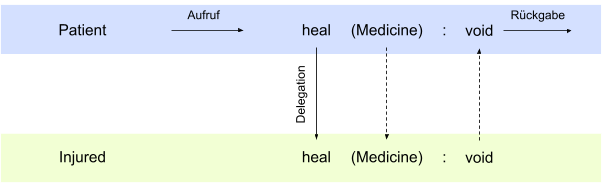
\includegraphics[width=\linewidth]{MDEL_heal}
\caption{Delegation der Methode $\texttt{heal}$}
\label{fig:DEL_heal}
\end{figure}
\noindent
An diesem Beispiel sind sowohl die Parameter- als auch die Rückgabe-Typen der aufgerufenen Methode und der Delegationsmethode identisch sind. Weiterhin spielt die Reihenfolge der Parameter in diesem Beispiel keine Rolle, da es nur einen Parameter gibt. Daher stellt die Übergabe der Parameter- und Rückgabewerte kein Problem dar.\\\\
Folgendes Beispiel soll zeigen, wie mit unterschiedlichen Reihenfolgen bzgl. der Parameter bei einer Methoden-Delegation umzugehen ist.
\paragraph{Beispiel} Die Methoden-Delegation aus Listing \ref{lst:methdel2} ist ein Beispiel für einen solchen Fall. Hier wird die aufgerufene Methode $\texttt{heal}$ mit den Parametern $\texttt{Patient}$ und $\texttt{MedCabinet}$ aus dem Typ $\texttt{PatientMedicalFireFighter}$ an die gleichnamige Methode aus dem Typ $\texttt{InverseDoctor}$ delegiert. Die Delegationsmethoden verwendet zwar identische Parameter-Typen, aber die Reihenfolge, in der die Parameter übergeben werden, ist unterschiedlich.
\begin{lstlisting}[style = dsl, caption = "Methoden-Delegation mit Parametern in unterschiedlicher Reihenfolge", captionpos = b]
	PatientMedicalFireFighter.heal(Patient, MedCabinet):void --> posModi(1,0)  InverseDoctor.heal(MedCabinet,Patient):void
\end{lstlisting}\label{lst:methdel2}
\noindent
Um die Reihenfolge der Parameter aus dem ursprünglichen Aufruf zu variieren, wird das Schlüsselwort $\texttt{posModi}$ verwendet. Dort werden eine Reihe von Indizes angegeben. Die Anzahl der angegebenen Indizes muss mit der Anzahl der Parameter übereinstimmen. Ein Index beschreibt die Position des in der aufgerufenen Methode angegebenen Parameter. Weiterhin spielt die Reihenfolge der Indizes eine wichtige Rolle. Diese ist mit der Reihenfolge der Parameter der Delegationsmethoden gleichzusetzen.\\\\
So wird in dem o.g. Beispiel der erste Parameter der aufgerufenen Methoden (Index = 0) der Delegationsmethode als zweiter Parameter übergeben. Dementsprechende wird er zweite Parameter der aufgerufenen Methoden (Index = 1) der Delegationsmethode als erster Parameter übergeben (siehe Abbildung \ref{fig:DEL_healInverse}). 
\begin{figure}[H]
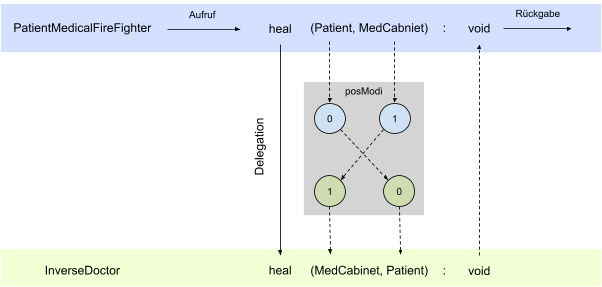
\includegraphics[width=\linewidth]{MDEL_healInverse}
\caption{Delegation der Methode $\texttt{heal}$ mit Parametern in unterschiedlicher Reihenfolge}
\label{fig:DEL_healInverse}
\end{figure}
\noindent
Ein weiteres Beispiel soll zeigen, wie mit übergebenen Typen umzugehen ist, die nicht ohne Probleme übergeben werden können. Dafür ist jedoch vorab zu klären, wann dies der Fall ist.\\\\
Dass identische Typen keine Probleme bei der Übergabe zwischen aufgerufener Methode und Delegationsmethode darstellen, wurde in den oben genannten Beispielen gezeigt.\\\\
Darüber hinaus können Typen aber auch dann ohne Probleme übergeben werden, wenn sie sich aufgrund des Substitutionsprinzips austauschen lassen. Unter Verwendung der in Abschnitt \ref{sec:matcher} beschriebenen Matcher sei dafür folgende Regeln definiert:
\begin{gather*}
\frac{T' \Rightarrow_{exact} T \vee T' \Rightarrow_{gen} T}{T' \Rightarrow_{exactGen} T }
\end{gather*}
\noindent
Bezogen auf das Substitutionsprinzip kann ein Typ $T$ anstelle eines Typs $T'$ verwendet werden, sofern $T' \Rightarrow_{exactGen} T$ gilt.
\paragraph{Beispiel} In Listing \ref{lst:methdel3} ist eine Methoden-Delegation aufgerührt, bei der sowohl die Parameter- als auch die Rückgabe-Typen der aufgerufenen Methode und der Delegationsmethode nicht auf Basis des Substitionsprinzips übergeben werden können.
\begin{lstlisting}[style = dsl, caption = "Methoden-Delegation mit Typkonvertierung", captionpos = b]
	MedicalFireFighter.extinguishFire(ExtFire):boolean --> FireFigher.extinguishFire(Fire):FireState
\end{lstlisting}\label{lst:methdel3}
\noindent
In einem solchen Fall müssen die Parameter-Typen der aufgerufenen Methoden in die Parameter-Typen der Delegationsmethode konvertiert werden. Analog dazu muss der Rückgabetyp der Delegationsmethode in den Rückgabetyp der aufgerufenen Methoden konvertiert werden.\\\\
Angenommen, die Funktion $\mathit{proxies(S,T)}$ beschreibt eine Menge von Proxies, mit $S$ als Source-Typ und $T$ als Menge der Target-Typen. Dann müssten bezogen auf die Methoden-Delegation aus Listing \ref{lst:methdel3} für die Parameter-Typen einer der Proxies aus der Menge $\mathit{proxies(\texttt{Fire}, \{\texttt{ExtFire}\})}$ an die Delegationsmethode übergeben werden. Nach der Ausführung der Delegationsmethode müsste ein Proxy aus der Menge $\mathit{proxies(\texttt{boolean},\{\texttt{FireState}\})}$ an die aufgerufenen Methode als Rückgabetyp übergeben werden. Der Sachverhalt wird in Abbildung \ref{fig:DEL_extinguishFire} schematisch dargestellt.
\begin{figure}[H]
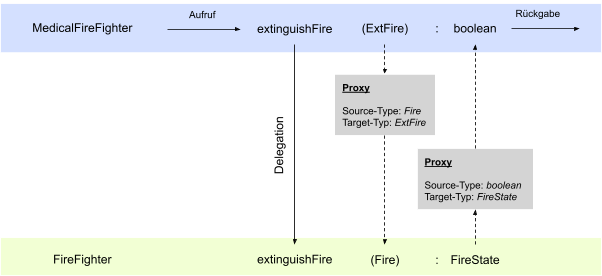
\includegraphics[width=\linewidth]{MDEL_extinguishFire}
\caption{Delegation der Methode $\texttt{extinguishFire}$ mit Typkonvertierungen}
\label{fig:DEL_extinguishFire}
\end{figure}
\noindent
Wie die Proxies generiert werden, wird im folgenden Abschnitt beschrieben.

\section{Generierung der Proxies auf Basis von Matchern}
Die Matcher beinhalten die Definition der jeweiligen Matchingrelation ($\Rightarrow$). Auf deren Basis werden Proxies für bestimmte Typen erzeugt. Dabei gibt es unterschiedliche Arten von Proxies. Jede Proxy-Art basiert auf einem anderen Matcher.\\\\
Wie im vorherigen Abschnitt bereits erwähnt, wird die Menge der Proxies für einen Source-Typ $S$ und einer Menge von Target-Typen $T$ über die Funktion $\mathit{proxies(S,T)}$ beschrieben. Für die unterschiedlichen Proxy-Arten gibt es ebenfalls Funktionen, die eine Menge von Proxies zu einem Source-Typen $S$ und einer Menge von Target-Typen $T$ beschreiben. Die Namen dieser Funktionen sind zusammen mit den Proxy-Arten und den dazugehörigen Matchingrelationen in Tabelle \ref{tab:baseMatcher} aufgeführt.

\begin{table}[H]
\centering
\begin{tabular}{|p{4cm}|p{4cm}|p{3cm}|}
\hline
\hline
\centering\textbf{Proxy-Art} & \textbf{Matchingrelation} & \textbf{Funktionsname}\\
\hline
\hline
Sub-Proxy
&  
$\Rightarrow_{spec}$
& 
$\mathit{proxy_{sub}}$
\\
\hline
Content-Proxy
& 
$\Rightarrow_{content}$
& 
$\mathit{proxy_{content}}$
\\
\hline
Container-Proxy
& 
$\Rightarrow_{container}$
& 
$\mathit{proxy_{container}}$
\\
\hline
struktureller Proxy
&
$\Rightarrow_{struct}$
& 
$\mathit{proxy_{struct}}$
 \\
\hline
\hline
\end{tabular}
\caption{Proxy-Arten mit Matchingrelationen und Funktionsnamen}
 \label{tab:baseMatcher}
\end{table}
\noindent
Die im vorherigen Abschnitt erwähnt Funktion $\mathit{proxy(S,T)}$ kann darauf aufbauend wie folgt beschrieben werden.
\begin{gather*}
\mathit{proxies(S,T)} := 
\left\{\begin{array}{ll}
\mathit{proxy_{sub}(S,T)}	& \text{wenn } |T| = 1 \wedge \mathit{ }\\
& \forall T' \in T. S \Rightarrow_{sub} T'\\	
&\\
\mathit{proxy_{content}(S,T)}	& \text{wenn } |T| = 1 \wedge \mathit{ }\\
& \forall T' \in T. S \Rightarrow_{content} T' \\
&\\
\mathit{proxy_{container}(S,T)} & \text{wenn } |T| = 1 \wedge \mathit{ } \\
& \forall T' \in T. S \Rightarrow_{container} T' \\
&\\
\mathit{proxy_{struct}(S,T)} & \text{wenn } |T| > 0 \wedge \mathit{ } \\
&\forall T' \in T. S \Rightarrow_{struct} T'
		 \end{array}
\right\}
\end{gather*}
\noindent
Die Proxies haben eine allgemeine Struktur, die in Abschnitt \ref{sec:proxygram} aufgeführt ist. Um die Regeln für die Generierung der Proxies zu beschreiben, soll davon ausgegangen werden, dass jedes Listen-Attribut aus Tabelle \ref{tab:attrGrProxies} ein Attribut $\texttt{len}$ enthält in dem die Anzahl der in der Liste befindlichen Elemente abgelegt ist.
\subsubsection{Sub-Proxy}
Die Voraussetzung für die Erzeugung eines \emph{Sub-Proxies} vom Typ $T$ aus einem Target-Typ $T'$ ist $T \Rightarrow_{spec} T'$. Damit ist der \emph{SpecTypeMatcher} der Basis-Matcher für den Sub-Proxy.\paragraph{Beispiel}
Als Beispiel soll hierfür der Typ $\texttt{Patient}$ als Source-Typ der Proxies und der Typ $\texttt{Injured}$ als Target-Typ verwendet werden. Da $\texttt{Patient} \Rightarrow_{spec} \texttt{Injured}$ gilt, kann ein \emph{Sub-Proxy} für diese Konstellation erzeugt werden. Der resultierende \emph{Sub-Proxy} ist im folgenden Listing aufgeführt.
\begin{lstlisting}[style = dsl]
proxy for Patient with [Injured]{
	Patient.heal(Medicine):void --> Injured.heal(Medicine):void
	Patient.getName():String --> err
}
\end{lstlisting}
Der abstrakte Syntaxbaum mit den dazugehörigen Attributen ist folgender Abbildung \ref{fig:ASTSUB} zu entnehmen. \footnote{Es wurden nur die Nonterminale mit den dazugehörigen Attributen aufgeführt.}
\begin{figure}[h!]
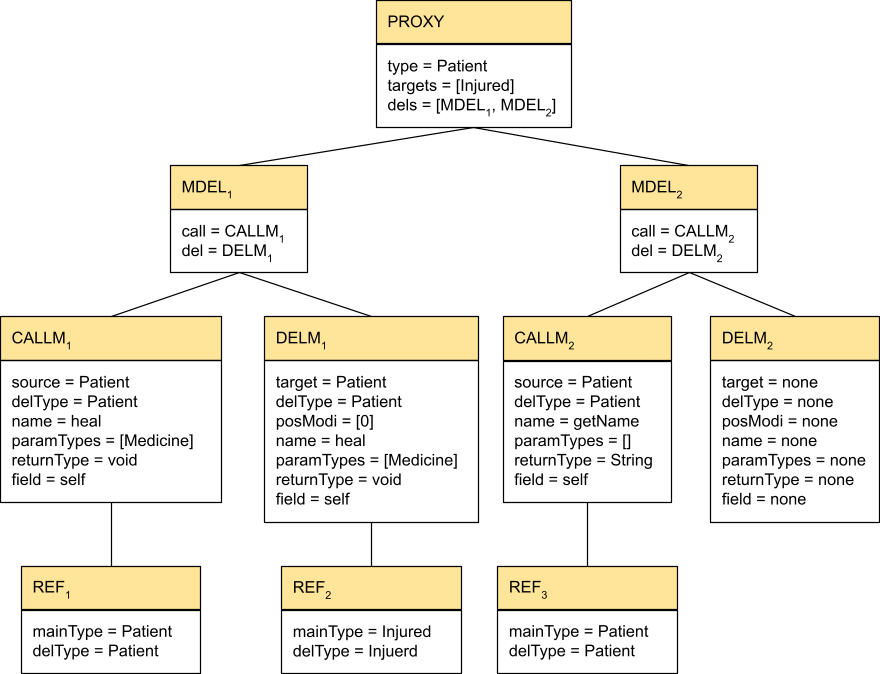
\includegraphics[width=\linewidth]{AST_SubExample}
\caption{AST für das Beispiel zum Sub-Proxy}
\label{fig:ASTSUB}
\end{figure}
\noindent
\paragraph{Formalisierung}
Wird der Proxy als Typ verwendet, so stehen darin alle Methoden zur Verfügung, die auch im Typ $\texttt{Patient}$ zur Verfügung stehen. Die Methodendelegationen innerhalb dieses Proxies, beschreiben, was beim Aufruf der jeweiligen aufgerufenen Methoden passiert. So wird ein Aufruf der Methode $\texttt{heal}$ an die Methode $\texttt{heal}$ aus dem Target-Typ delegiert. Ein Aufruf der Methode $\texttt{getName}$ hingegen führt zu einem Fehler, weil keine Delegationsmethode zur Verfügung steht.\\\\
In Hinblick darauf, dass eine Konvertierung von einem Super-Typ und einen Sub-Typ (Down-Cast) ebenfalls dazu führt, dass bestimmte Methoden, wie in diesem Fall $\texttt{getName}$ nicht ausgeführt werden kann, spiegelt der \emph{Sub-Proxy} dieses Verhalten wieder.\\\\
Formal wird ein \emph{Sub-Proxy} durch die Regeln beschrieben, die im Folgenden vorgestellt werden.
Ein \emph{Sub-Proxy} enthält genau einen Target-Typ. Für einen Proxy $P$ wird dieser Sachverhalt durch die folgende Regel dargestellt.
\begin{gather*}
\frac{|P.targets| = 1 \wedge P.targets[0] = T'}{\mathit{singleTarget(T')}}
\end{gather*}
Darüber hinaus enthält ein \emph{Sub-Proxy} $P$ eine bestimmte Menge von Methoden-Delegationen. Dabei muss das Attribut $\texttt{field}$ sowohl in den aufgerufenen Methoden und in den Delegationsmethoden aller Methodendelegationen jeweils übereinstimmen. Folgende Regel stellt diesen Sachverhalt für eine Menge von Methodendelegationen $\mathit{MDEL}$ dar.
\begin{gather*}
\frac{\splitfrac{\forall \mathit{DEL_1}\in \mathit{MDEL}. \neg(\exists \mathit{DEL_2} \in \mathit{MDEL}.DEL_1.call.field \neq DEL_2.call.field}{ \vee DEL_1.del.field \neq DEL_2.del.field )}}
{\mathit{equalRefs(MDEL)}}
\end{gather*}
Für jede einzelne Methoden-Delegation gilt weiterhin, dass die aufgerufenen Methode und die Delegationsmethode denselben Namen haben.
\begin{gather*}
\frac{\mathit{DEL.call.name} = \mathit{DEL.del.name}}
{\mathit{nominalDel(DEL)}}
\end{gather*}
Die aufgerufene Methode muss dabei generell im Typ aus dem Attribut $call.declType$ deklariert sein und die Delegationsmethode im Typ aus dem Attribut $del.declType$.
\begin{gather*}
\frac{\exists m(P_1,...,P_n):R \in \mathit{methoden(DEL.call.declType)}. \mathit{DEL.call.name} = m}
{\mathit{simpleCallMethod(DEL, P)}}
\end{gather*}
\begin{gather*}
\frac{\exists m(P_1,...,P_n):R \in \mathit{methoden(DEL.del.declType)}. \mathit{DEL.del.name} = m}
{\mathit{simpleDelMethod(DEL, P)}}
\end{gather*}
Zusätzlich muss das Attribut $\texttt{field}$ sowohl im Attribut $call$ mit dem Wert $\texttt{self}$ belegt und das Attribut $\texttt{mainType}$ mit dem Typ des Proxies belegt sein.
\begin{gather*}
\frac{\mathit{DEL.call.mainType} = \mathit{P.type} \wedge \mathit{DEL.call.field} = \mathit{self}}
{\mathit{simpleDelSource(DEL, P)}}
\end{gather*}
Damit ist auch gewährleistet, dass die Attribute $\texttt{mainType}$ und $\texttt{delType}$ im Attribut $\texttt{call}$ übereinstimmen.\\\\
Ähnliches gilt für die Attribute $\texttt{field}$ und $\texttt{mainType}$ im Attribut $del$. Hierbei muss der Wert des Attributs $\texttt{mainType}$ jedoch mit dem Target-Typ des Proxies übereinstimmen.
\begin{gather*}
\frac{\mathit{DEL.del.mainType} = \mathit{P.targets[0]}\wedge \mathit{DEL.del.field} = \mathit{self}}
{\mathit{simpleDelTarget(DEL, P)}}
\end{gather*}
Damit ist wiederum gewährleistet, dass die Attribute $\texttt{mainType}$ und $\texttt{delType}$ im Attribut $\texttt{del}$ übereinstimmen.\\\\
Die Regeln bzgl. der linken Seite einer Methoden-Delegation innerhalb eines \emph{Sub-Proxies} können damit in folgender Regel zusammengefasst werden:
\begin{gather*}
\frac{\mathit{simpleCallMethod(DEL,P)} \wedge \mathit{simpleDelSource(DEL,P)}}
{simpleCall(DEL,P)}
\end{gather*}
Analog dazu können auch die Regeln bzgl. der rechten Seite einer Methoden-Delegation innerhalb eines \emph{Sub-Proxies} zusammengefasst werden:
\begin{gather*}
\frac{\mathit{simpleDelMethod(DEL,P)} \wedge \mathit{simpleDelTarget(DEL,P)}}
{simpleDel(DEL,P)}
\end{gather*}
Jedoch ist im \emph{Sub-Proxy} die Ausnahme zu beachten:
\begin{gather*}
\frac{\mathit{DEL.del.name} = \mathit{none}}
{\mathit{errDel(DEL)}}
\end{gather*}
In diesem Fall würden die o.g. Kriterien nicht gelten. Die genannten Regeln bzgl. einer Methoden-Delegation in einem \emph{Sub-Proxy} lassen sich über beiden folgenden Regeln beschreiben:
\begin{gather*}
\frac{\mathit{simpleCall(DEL,P)} \wedge \mathit{simpleDel(DEL,P) \wedge \mathit{nominalDel(DEL)}}}
{subDelegation(DEL,P)}
\end{gather*}
\begin{gather*}
\frac{\mathit{simpleCall(DEL,P)}\wedge\mathit{errDel(DEL)}
}
{subMDEL(DEL,P)}
\end{gather*}
Innerhalb eines \emph{Sub-Proxies} gibt es für jede Methode $m$ des Source-Typ genau eine Methoden-Delegation, mit der Methode $m$ als aufgerufene Methode. Damit lässt sich für einen Proxy $P$ in Bezug auf seine Methoden-Delegationen folgende Regeln formulieren:
\begin{gather*}
\frac{\splitfrac{|\mathit{methoden(P.type)}| = |P.dels| \wedge}{ \splitfrac{\forall m(P_1,...,P_n):R \in \mathit{methoden(P.type)}.\exists DEL \in P.dels.}{m = \mathit{DEL.call.name} \wedge \mathit{subMDEL(DEL,P)}
 }}
}
{subMDELList(P)}
\end{gather*}
Die Menge der \emph{Sub-Proxies}, die mit dem Source-Typ $T$ und dem Target-Typ $T'$ erzeugt werden, wird durch die folgende Funktion beschrieben.
\begin{gather*}
\mathit{proxies_{sub}(T,T')} := 
\left\{\begin{array}{l|l}
	P	& P\texttt{.type} = T \wedge  \mathit{singleTarget(T')} \wedge \mathit{ }\\
		& \mathit{equalRefs(P.dels)} \wedge \mathit{subMDELList(P)}
		 \end{array}
\right\}
\end{gather*}


\subsubsection{Content-Proxy}
Die Voraussetzung für die Erzeugung eines \emph{Content-Proxies} vom Typ $T$ aus einem Target-Typ $T'$ ist $T \Rightarrow_{content} T'$. Damit ist der \emph{ContentTypeMatcher} der Basis-Matcher für den \emph{Content-Proxy}.
\paragraph{Beispiel} Als Beispiel können hierfür die Typen $\texttt{Medicine}$ und $\texttt{MedCabinet}$ verwendet werden. Diese weisen ein Matching der Form $texttt{Medicine} \Rightarrow_{content} texttt{MedCabinet}$ auf. Daher kann ein \emph{Content-Proxy} für diese Konstellation erzeugt werden. Ein resultierender \emph{Content-Proxy} ist in folgendem Listing aufgeführt.
\begin{lstlisting}[style = dsl]
proxy for Medicine with [MedCabinet]{
	Medicine.getDesciption():String --> MedCabinet.med.getDesciption():String
}
\end{lstlisting}
Durch die Methoden-Delegation dieses \emph{Content-Proxies} wird die Methode $\texttt{getDescription}$ an das Feld $\texttt{med}$ des Target-Typen $\texttt{MedCabniet}$ delegiert.\\\\
Der abstrakte Syntaxbaum mit den dazugehörigen Attributen ist folgender Abbildung \ref{fig:ASTCONTENT} zu entnehmen. \footnote{Es wurden nur die Nonterminale mit den dazugehörigen Attributen aufgeführt.}
\begin{figure}[h!]
\centering
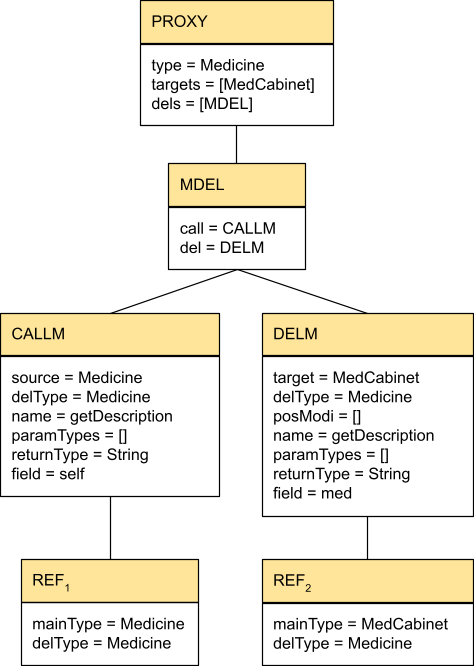
\includegraphics[width=0.5\linewidth]{AST_ContentExample}
\caption{AST für das Beispiel zum Content-Proxy}
\label{fig:ASTCONTENT}
\end{figure}
\noindent
\paragraph{Formalisierung}
Formal wird ein \emph{Content-Proxy} durch die Regeln beschrieben, die im Folgenden vorgestellt werden.\\\\
Ein \emph{Content-Proxy} enthält, wie auch der \emph{Sub-Proxy}, genau einen Target-Typ. Ebenfalls identisch zum \emph{Sub-Proxy} sind die Bedingungen hinsichtlich der aufgerufenen Methoden in den einzelnen Methoden-Delegationen.\\\\
In den Delegationsmethoden einer einzelnen Methoden-Delegation darf das Attribut $\texttt{mainType}$ und $\texttt{delType}$ im \emph{Content-Proxy} nicht identisch sein. Dementsprechend darf das Attribut $\texttt{field}$ nicht mit dem Wert $\texttt{self}$ belegt sein. Vielmehr muss für das Attribut $\texttt{delTyp}$ und den Source-Typ $T$ im Attribut $\texttt{type}$ des Proxies ein Matching der Form $T \Rightarrow_{internCont} \texttt{delTyp}$ gelten. Daher gilt für den \emph{Content-Proxy} folgende Regel.
\begin{gather*}
\frac{\mathit{DEL.del.mainType} = \mathit{P.targets[0]} \wedge \mathit{P.type} \Rightarrow_{internCont} \mathit{DEL.del.delType}}
{\mathit{contentDelTarget(DEL,P)}}
\end{gather*}
\noindent
Damit ist auch die zusammenfassende Regel für die Delegationsmethoden eine andere:
\begin{gather*}
\frac{\mathit{simpleDelMethod(DEL,P)} \wedge \mathit{contentDelTarget(DEL,P)}}
{contentDel(DEL,P)}
\end{gather*}
Die zusammenfassende Regel für eine einzelne Methoden-Delegation innerhalb eines \emph{Content-Proxies} hat die folgende Form:
\begin{gather*}
\frac{\mathit{simpleCall(DEL,P)} \wedge \mathit{contentDel(DEL,P) \wedge \mathit{nominalDel(DEL)}}}
{contentMDEL(DEL,P)}
\end{gather*}
Wie auch im \emph{Sub-Proxy} gibt es im \emph{Content-Proxy} für jede Methode $m$ des Source-Typen genau eine Methoden-Delegation mit der Methode $m$ als aufgerufene Methode. Daraus ergibt sich für alle Methoden-Delegationen aus einem \emph{Content-Proxy} $P$ folgende Regel:
\begin{gather*}
\frac{\splitfrac{|\mathit{methoden(P.type)}| = |P.dels| \wedge}{ \splitfrac{\forall m(P_1,...,P_n):R \in \mathit{methoden(P.type)}.\exists DEL \in P.dels.}{m = \mathit{DEL.call.name} \wedge \mathit{contentMDEL(DEL,P)}
 }}
}
{contentMDELList(P)}
\end{gather*}
Die Menge der \emph{Content-Proxies}, die mit dem Source-Typ $T$ und dem Target-Typ $T'$ erzeugt werden, wird durch die folgende Funktion beschrieben.
\begin{gather*}
\mathit{proxies_{content}(T,T')} := 
\left\{\begin{array}{l|l}
	P	& P\texttt{.type} = T \wedge  \mathit{singleTarget(T')} \wedge \mathit{ }\\
		& \mathit{equalRefs(P.dels)} \wedge \mathit{contentMDELList(P)} 
		 \end{array}
\right\}
\end{gather*}
\subsubsection{Container-Proxy}
Die Voraussetzung für die Erzeugung eines \emph{Container-Proxies} vom Typ $T$ aus einem Target-Typ $T'$ ist $T \Rightarrow_{container} T'$. Damit ist der \emph{ContainerTypeMatcher} der Basis-Matcher für den \emph{Container-Proxy}.
\paragraph{Beispiel}
Als Beispiel können hierfür wiederum die Typen $\texttt{Medicine}$ und $\texttt{MedCabinet}$ verwendet werden. Diese weisen ein Matching der Form $\texttt{MedCabinet} \Rightarrow_{container} \texttt{Medicine}$ auf. Daher kann ein \emph{Content-Proxy} für diese Konstellation erzeugt werden. Ein resultierender \emph{Content-Proxy} ist in folgendem Listing aufgeführt.
\begin{lstlisting}[style = dsl]
proxy for MedCabinet with [Medicine]{
	MedCabinet.med.getDesciption():String --> Medicine.getDesciption():String
}
\end{lstlisting}
Durch die Methoden-Delegation dieses \emph{Container-Proxies} findet eine Delegation nur dann statt, wenn die Methoden $\texttt{getDescription}$ auf dem Feld $\texttt{med}$ des Source-Typ aufgerufen wird. Diese wird dann an den Target-Typen $\texttt{MedCabniet}$ delegiert.\\\\
Der abstrakte Syntaxbaum mit den dazugehörigen Attributen ist folgender Abbildung \ref{fig:ASTCONTAINER} zu entnehmen. \footnote{Es wurden nur die Nonterminale mit den dazugehörigen Attributen aufgeführt.}
\begin{figure}[h!]
\centering
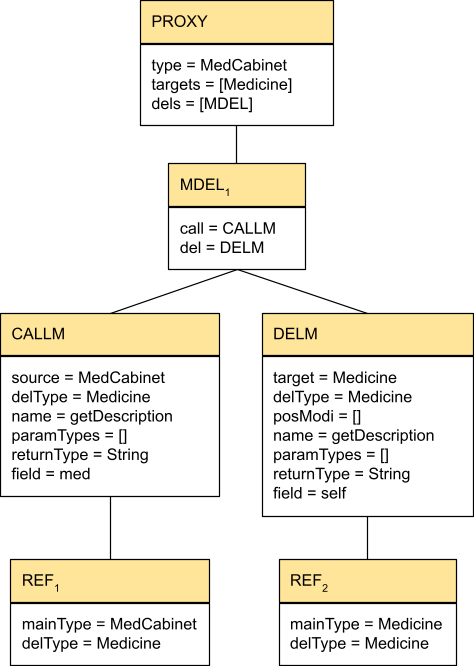
\includegraphics[width=0.5\linewidth]{AST_ContainerExample}
\caption{AST für das Beispiel zum Container-Proxy}
\label{fig:ASTCONTAINER}
\end{figure}
\noindent
\paragraph{Formalisierung}
Formal wird ein \emph{Container-Proxy} durch die Regeln beschrieben, die im Folgenden vorgestellt werden.\\\\
Ein \emph{Container-Proxy} enthält, wie die vorher beschriebenen Proxies , genau einen Target-Typ. Die Eigenschaften der einzelnen Delegationsmethoden gleichen denen aus dem \emph{Sub-Proxy}.\\\\
In den angerufenen Methoden einer einzelnen Methoden-Delegation dürfen die Attribute $\texttt{mainType}$ und $\texttt{delType}$ im \emph{Container-Proxy} nicht übereinstimmen. Dementsprechend darf das Attribut $\texttt{field}$ nicht mit dem Wert $\texttt{self}$ belegt sein. Vielmehr muss für das Attribut $\texttt{delTyp}$ und den Target-Typ $T$ ein Matching der Form $T \Rightarrow_{internCont} \texttt{delTyp}$ gelten. Daher gilt für den \emph{Container-Proxy} folgende Regel.
\begin{gather*}
\frac{\mathit{DEL.call.mainType} = \mathit{P.type} \wedge \mathit{P.targets[0]} \Rightarrow_{internCont} \mathit{DEL.call.delType}}
{\mathit{containerDelSource(DEL,P)}}
\end{gather*}
\noindent
Damit ist auch die zusammenfassende Regel für die aufgerufenen Methoden eine andere:
\begin{gather*}
\frac{\mathit{simpleCallMethod(DEL,P)} \wedge \mathit{containerDelSource(DEL,P)}}
{containerCall(DEL,P)}
\end{gather*}
Die zusammenfassende Regel für eine einzelne Methoden-Delegation innerhalb eines \emph{Container-Proxies} hat die folgende Form:
\begin{gather*}
\frac{\mathit{containerCall(DEL,P)} \wedge \mathit{simpleDel(DEL,P) \wedge \mathit{nominalDel(DEL)}}}
{containerMDEL(DEL,P)}
\end{gather*}
Für einen \emph{Container-Proxy} $P$ gilt ebenfalls die Regel $\mathit{equalRefs(P.dels)}$. Daher müssen die Werte des Attributs $\texttt{call.delType}$ aller Methoden-Delegationen des Proxies $P$ übereinstimmen. Ferner muss es für jede Methode $m$ des Typen aus $\texttt{call.delType}$ genau eine Methoden-Delegation mit der Methode $m$ als aufgerufene Methode. Daraus ergibt sich für alle Methoden-Delegationen aus einem \emph{Content-Proxy} $P$ folgende Regel:
\begin{gather*}
\frac{\splitfrac{|\mathit{methoden(P.dels[0].call.delType)}| = |P.dels| \wedge}{ \splitfrac{\forall m(P_1,...,P_n):R \in \mathit{methoden(P.dels[0].call.delType)}.}{\exists DEL \in P.dels.m = \mathit{DEL.call.name} \wedge \mathit{containerMDEL(DEL,P)}
 }}
}
{\mathit{containerMDELList(P)}}
\end{gather*}
Die Menge der \emph{Container-Proxies}, die mit dem Source-Typ $T$ und dem Target-Typ $T'$ erzeugt werden, wird durch die folgende Funktion beschrieben.
\begin{gather*}
\mathit{proxies_{container}(T,T')} := 
\left\{\begin{array}{l|l}
	P	& P\texttt{.type} = T \wedge  \mathit{singleTarget(T')} \wedge \mathit{ }\\
		& \mathit{equalRefs(P.dels)} \wedge \mathit{containerMDELList(P)} 
		 \end{array}
\right\}
\end{gather*}

\subsubsection{Struktureller Proxy}
Die Voraussetzung für die Erzeugung eines \emph{strukturellen Proxies} vom \emph{required Typ} $R$ aus einem Target-Typ $T$ ist $R \Rightarrow_{struct} T$. Damit ist der \emph{StructuralTypeMatcher} der Basis-Matcher für den \emph{strukturellen Proxy}.\\\\
Der \emph{strukturelle Proxy} ist der einzige Proxy, der mit mehreren Target-Typen erzeugt werden kann. 
\paragraph{Beispiel}
Als Beispiel hierfür können die Typen $MedicalFireFighter$, $Doctor$ und $FireFighter$ verwendet werden. Dabei ist $MedicalFireFighter$ der Source-Typ des Proxies und die Menge der anderen beiden Typen bilden die Target-Typen des Proxies.
\begin{lstlisting}[style = dsl]
proxy for MedicalFireFighter with [Doctor, FireFighter]{
	MedicalFireFighter.heal(Patient, MedCabinet):void --> Doctor.heal(Patient, Medicine):void
	MedicalFireFighter.extinguishFire(ExtFire):boolean --> FireFighter.extinguishFire(Fire):FireState
}
\end{lstlisting}
In diesem Beispiel wird der Methodenaufruf der Methode $\texttt{heal}$ auf dem Proxy an die Methode $heal$ des Typs $Doctor$ delegiert. Analog dazu würde ein Aufruf der Methode $\texttt{extinguishFire}$ auf dem Proxy an die Methode $extinguishFire$ des Typs $FireFighter$ delegiert werden. Die Methoden stimmen jeweils strukturell überein.\\\\
Der abstrakte Syntaxbaum mit den dazugehörigen Attributen ist folgender Abbildung \ref{fig:ASTSTRUCT} zu entnehmen. \footnote{Es wurden nur die Nonterminale mit den dazugehörigen Attributen aufgeführt.}
\begin{figure}[h!]
\centering
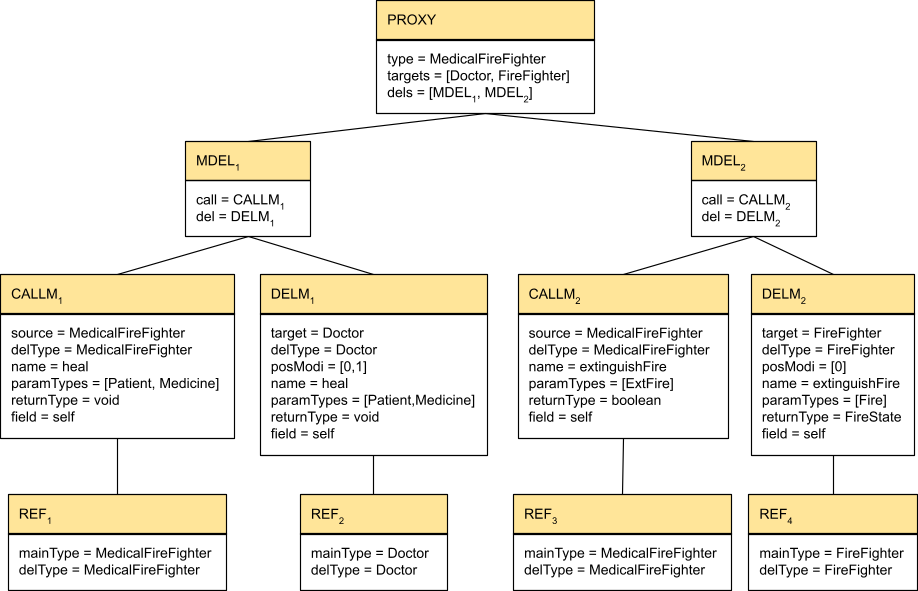
\includegraphics[width=\linewidth]{AST_StructExample}
\caption{AST für das Beispiel zum strukturellen Proxy}
\label{fig:ASTSTRUCT}
\end{figure}
\noindent
\paragraph{Formalisierung}
Ein \emph{struktureller Proxy} wird formal durch die folgenden Regeln beschrieben.\\\\
Ein \emph{struktureller Proxy} kann, wie bereits erwähnt, mehrere Target-Typen enthalten.
Für jeden Target-Typ $T$ muss dabei jedoch wenigstens eine Delegationsmethode im Proxy mit einem Attribut $\texttt{target} = T$ existiert. Dadurch gilt die für einen \emph{strukturellen Proxy} Proxy $P$:
\begin{gather*}
\frac{\forall T \in \mathit{P.targets}.\exists \mathit{MDEL} \in \mathtt{P.dels}.\mathit{MDEL.del.target} = T}{\mathit{structTargets(P)}}
\end{gather*}
Für die aufgerufene Methode und die Delegationsmethode einer einzelnen Methoden-Delegation $\mathit{DEL}$ gelten im \emph{strukturellen Proxy} dieselben Regeln wie für den \emph{Sub-Proxy}. Die Namen der aufgerufenen Methode und der Delegationsmethode müssen dabei nicht übereinstimmen. Dafür müssen diese beiden Methode jedoch ein strukturelles Matching aufweisen. Bezogen auf die Rückgabe-Typen einer aufgerufenen Methode $\mathit{CALL}$ und der Delegationsmethode $\mathit{DELM}$ aus einer Methodendelegation muss daher Folgendes gelten.
\begin{gather*}
\frac{\mathit{DELM.returnType} \Rightarrow_{internStruct} \mathit{CALL.returnType}}{\mathit{structRT(CALL, DELM)}}
\end{gather*} 
Weiterhin muss für die Parameter-Typen gelten:
\begin{gather*}
\frac{\mathit{CALL.paramCount} = 0}{\mathit{structParams(CALL, DELM)}}
\end{gather*} 
\begin{gather*}
\frac{\splitfrac{\forall i \in \{0,...,\mathit{CALL.paramCount}-1\}.}
{ \mathit{CALL.paramTypes}[i] \Rightarrow_{internStruct} \mathit{DELM.paramTypes}[\mathit{DELM.posModi}[i]]
}}{\mathit{structParams(CALL, DELM)}}
\end{gather*} 
Für eine einzelnen Methoden-Delegation $\mathit{MDEL}$ eines \emph{strukturellen Proxies} $P$ kann dann folgende Regel aufgestellt werden.
\begin{gather*}
\frac{\splitfrac{\mathit{simpleCall(MDEL,P)} \wedge \mathit{simpleDel(MDEL,P)} \wedge} {\mathit{structRT(MDEL.call, MDEL.del)} \wedge \mathit{structParams(MDEL.call, MDEL.del)}}
}
{\mathit{structMDEL(MDEL, P)}}
\end{gather*}
Für einen \emph{strukturellen Proxy} $P$ gilt ebenfalls die Regel $\mathit{equalRefs(P.dels)}$. Daher müssen die Werte des Attributs $\texttt{call.delType}$ aller Methoden-Delegationen des Proxies $P$ übereinstimmen.\\\\
Für jede Methode $m$ des Source-Typen genau eine Methoden-Delegation mit der Methode $m$ als aufgerufene Methode. Daraus ergibt sich für alle Methoden-Delegationen aus einem \emph{strukturellen Proxy} $P$ folgende Regel:
\begin{gather*}
\frac{\splitfrac{|\mathit{methoden(P.type)}| = |P.dels| \wedge}{ \splitfrac{\forall m(P_1,...,P_n):R \in \mathit{methoden(P.type)}.}{\exists DEL \in P.dels.m = \mathit{DEL.call.name} \wedge \mathit{structMDEL(DEL,P)}
 }}
}
{\mathit{structMDELList(P)}}
\end{gather*}
Die Menge der \emph{strukturellen Proxies}, die mit dem Source-Typ $R$ und der Menge von Target-Typen $T$ erzeugt werden, wird durch die folgende Funktion beschrieben.
\begin{gather*}
\mathit{proxies_{struct}(R,T)} := 
\left\{\begin{array}{l|l}
	P	& P\texttt{.type} = R \wedge  \mathit{structTargets(P)} \wedge \mathit{ }\\
		& \mathit{equalRefs(P.dels)} \wedge \mathit{structMDELList(P)} 
		 \end{array}
\right\}
\end{gather*}

\subsubsection{Mögliche Proxies in eine Bibliothek}
Innerhalb einer Bibliothek $L$ können für einen \emph{required Typ} $R$ mitunter eine Vielzahl von \emph{strukturellen Proxies} erzeugt werden. Die Anzahl hängt zum einen von der Anzahl der Mengen von \emph{provided Typen} $T$ ab, mit denen ein solcher \emph{struktureller Proxie} erzeugt werden kann.\\\\
Die folgende Funktion $\mathit{cover}$ beschreibt die eine Menge von Mengen von \emph{provided Typen} aus einer Bibliothek $L$, die für die Erzeugung eines \emph{strukturellen Proxies} für $R$ verwendet werden können.
\begin{gather*}
cover(R,L) := 
\left\{\begin{array}{l|l}
					& T_1 \in L \wedge \text{...} \wedge T_n \in L \wedge \\
					& methoden(R) = structM(R,T_1) \cup \\
	\{T_1,...,T_n\}	& \texttt{...} \cup structM(R, T_n) \wedge \\
					& \mathit{structM(R,T_1)} \neq \emptyset \wedge \\
					& \texttt{...}\wedge \mathit{structM(R,T_n)} \neq \emptyset 
\end{array}\right\}
\end{gather*}
Darüber hinaus können zu einer Menge aus $\mathit{cover(R,L)}$ durchaus mehrere \emph{strukturelle Proxies} erzeugt werden. Das ist dann der Fall, wenn mehrere der Methoden aus den \emph{provided Typen} mit einer Methode aus dem \emph{required Typ} strukturell übereinstimmen. 


\end{document}